% TS-DDR training with a deterministic-equivalent second stage.
%
% This is a redraw of the published TS-DDR figure (Fig. 1 of arXiv:2405.14973,
% formerly diagram_tsddr.png in this repository). The content is the published
% figure's: a sampled uncertainty, per-stage policies emitting state targets,
% ONE deterministic-equivalent problem over the horizon in which the targets
% enter as parameters, the dual of the target constraints from duality, and the
% automatic-differentiation chain back to the policy weights. Only the visual
% style changed (colours, shapes and lane titles). Notation follows README.md.
%
% Build (from this directory):
%   pdflatex tsddr.tex                          -> wide layout   (tsddr.pdf)
%   pdflatex -jobname=tsddr-compact tsddr.tex   -> narrow layout (tsddr-compact.pdf)
% then ../build.sh converts both to SVG with a white background.
\documentclass[tikz,border=4pt]{standalone}
\usepackage{amsmath,amssymb,bm}
\usepackage[T1]{fontenc}
\usepackage[scaled=0.92]{helvet}
\renewcommand{\familydefault}{\sfdefault}
\usetikzlibrary{arrows.meta,shapes.geometric,shapes.symbols,calc,positioning,decorations.pathreplacing}

\definecolor{dTeal}{HTML}{1A9AA0}
\definecolor{dTealLine}{HTML}{3FB3B8}
\definecolor{dNavy}{HTML}{3F4C8C}
\definecolor{dInk}{HTML}{1E2235}
\definecolor{dRed}{HTML}{E4573D}
\definecolor{dCoral}{HTML}{E2765A}
\definecolor{dOrange}{HTML}{F4A93B}
\definecolor{dPeach}{HTML}{FBD9AC}
\definecolor{dPanel}{HTML}{EEF0F2}
\definecolor{dGray}{HTML}{8A90A0}
\definecolor{dNode}{HTML}{14A3A8}
\definecolor{dShadow}{HTML}{D5DAE3}

\newcommand{\xh}{\hat{x}}
\newcommand{\pol}{\pi_t(\{w_j\}_{j=2..t},\,x_0;\,\theta_t)}
\newcommand{\polT}{\pi(\{w_j\}_{j=2..T},\,x_0;\,\theta)}

\newif\ifcompact
\edef\compactname{\detokenize{tsddr-compact}}
\edef\jobstr{\jobname}
\ifx\jobstr\compactname\compacttrue\fi

\tikzset{
  >={Stealth[length=5pt,width=4pt]},
  every node/.style={text=dInk},
  title/.style={anchor=west,font=\small,inner sep=0pt},
  note/.style={font=\itshape\footnotesize,text=dNavy},
  dnote/.style={font=\itshape\footnotesize,text=dCoral},
  store/.style={cylinder,shape border rotate=90,aspect=0.28,fill=dPeach,draw=dOrange,
                line width=0.7pt,minimum width=0.95cm,minimum height=1.2cm,font=\normalsize},
  dia/.style={diamond,fill=dOrange,draw=none,minimum size=0.9cm,inner sep=0pt,aspect=1,
              font=\normalsize},
  lnode/.style={circle,fill=dRed,draw=none,minimum size=0.66cm,inner sep=0pt,
                text=white,font=\normalsize},
  card/.style={rectangle,rounded corners=4pt,fill=white,draw=dShadow,line width=0.6pt},
  sheet/.style={rectangle,rounded corners=3pt,fill=dPanel,draw=dShadow,line width=0.6pt},
  fwd/.style={->,dTealLine,line width=0.8pt},
  tgt/.style={->,dOrange,line width=0.9pt},
  dual/.style={->,dCoral,dashed,line width=0.9pt},
  nn/.style={circle,minimum size=0.26cm,inner sep=0pt,draw=dInk!70,line width=0.35pt},
}

% Lane frame in the paper style: two shadow copies behind a teal rounded frame.
\newcommand{\lane}[4]{% #1 x0, #2 y0, #3 x1, #4 y1
  \foreach \o/\c in {0.16/dShadow!60,0.08/dShadow}
    \draw[\c,fill=white,rounded corners=5pt,line width=0.6pt]
      (#1+\o,#2-\o) rectangle (#3+\o,#4-\o);
  \draw[dTealLine,fill=white,rounded corners=5pt,line width=0.9pt] (#1,#2) rectangle (#3,#4);}

% Per-stage policy: stacked sheets (one per stage t) with a network drawing on
% the front one. #1 = centre of the front sheet, #2 = name prefix.
\newcommand{\policy}[2]{%
  \begin{scope}[shift={(#1)}]
    \node[sheet,minimum width=2.1cm,minimum height=2.05cm] at (0.30,0.22) {};
    \node[sheet,minimum width=2.1cm,minimum height=2.05cm] at (0.15,0.11) {};
    \node[sheet,minimum width=2.1cm,minimum height=2.05cm,fill=white] (#2sheet) at (0,0) {};
    \foreach \y [count=\i] in {0.42,0,-0.42} \node[nn,fill=dGray!45] (#2in\i) at (-0.72,\y) {};
    \foreach \y [count=\i] in {0.66,0.33,0,-0.33,-0.66} \node[nn,fill=dNode] (#2ha\i) at (-0.24,\y) {};
    \foreach \y [count=\i] in {0.5,0.17,-0.17,-0.5} \node[nn,fill=dNode] (#2hb\i) at (0.24,\y) {};
    \node[nn,fill=dOrange] (#2out) at (0.72,0) {};
    \foreach \a in {1,...,3} \foreach \b in {1,...,5} \draw[dGray!60,line width=0.2pt] (#2in\a) -- (#2ha\b);
    \foreach \a in {1,...,5} \foreach \b in {1,...,4} \draw[dGray!60,line width=0.2pt] (#2ha\a) -- (#2hb\b);
    \foreach \a in {1,...,4} \draw[dGray!60,line width=0.2pt] (#2hb\a) -- (#2out);
    \node[font=\footnotesize\itshape,text=dNavy] at (-0.82,-0.82) {$t$};
  \end{scope}}

\newcommand{\problem}{%
  $\begin{aligned}
    \min_{x,\,y,\,\delta}\;\; & Q(w,\xh)=\sum_{t} f(x_t,y_t)+C_\delta\|\delta_t\| \\[2pt]
    \text{s.t.}\;\; & x_t=\mathcal{T}(x_{t-1},{\color{dRed}w_t},y_t) && \forall t\\[2pt]
    & x_t+\delta_t={\color{dRed}\xh_t}\quad{\color{dRed}:\;\lambda_t} && \forall t\\[2pt]
    & h(x_t,y_t)\ge 0 && \forall t
  \end{aligned}$}

\begin{document}
\ifcompact
% ============================ narrow (phone) layout ============================
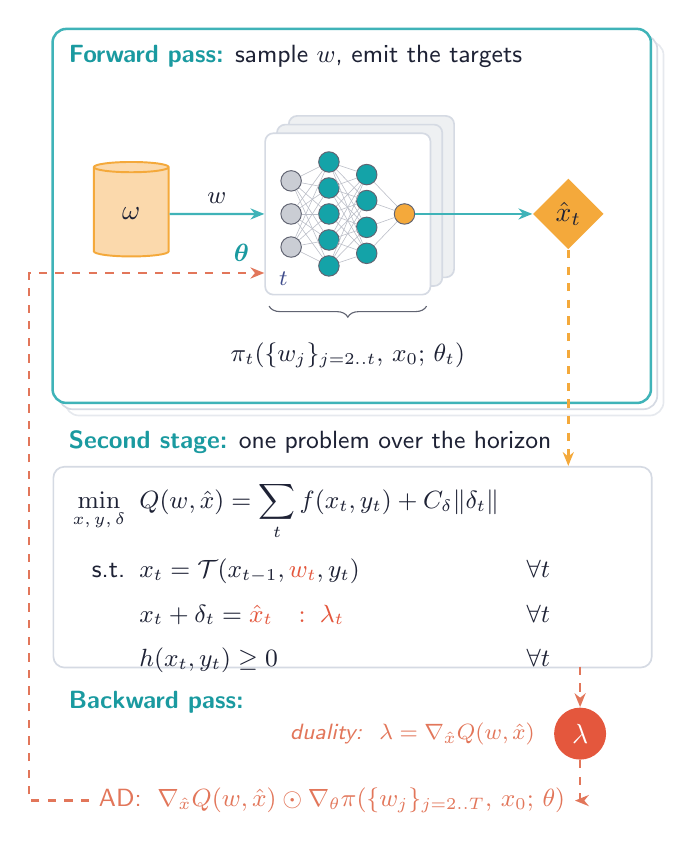
\begin{tikzpicture}
  % forward pass
  \lane{0}{4.95}{7.6}{9.7}
  \node[title] at (0.2,9.35) {\textcolor{dTeal}{\bfseries Forward pass:} sample $w$, emit the targets};
  \node[store] (om) at (1.0,7.35) {$\omega$};
  \policy{3.75,7.35}{p}
  \draw[fwd] (om.east) -- node[above,font=\small] {$w$} (pin2.west -| psheet.west);
  \node[dia] (xh) at (6.55,7.35) {$\xh_t$};
  \draw[fwd] (pout.east) -- (xh.west);
  \draw[decorate,decoration={brace,mirror,amplitude=4pt},dInk!70] (2.75,6.18) -- (4.75,6.18);
  \node[font=\small] at (3.75,5.55) {$\pol$};
  % the deterministic equivalent
  \node[title] at (0.2,4.45) {\textcolor{dTeal}{\bfseries Second stage:} one problem over the horizon};
  \node[card,minimum width=7.6cm,minimum height=2.55cm,anchor=north west] (de) at (0,4.15) {};
  \node[anchor=north west,font=\small,inner sep=0pt] at (0.25,3.95) {\problem};
  \draw[tgt,dashed] (xh.south) -- (6.55,4.15);
  % backward pass
  \node[title] at (0.2,1.15) {\textcolor{dTeal}{\bfseries Backward pass:}};
  \node[lnode] (lam) at (6.7,0.75) {$\lambda$};
  \draw[dual] (6.7,1.6) -- (lam.north);
  \node[dnote,anchor=east] at (6.25,0.75) {duality:\; $\lambda=\nabla_{\xh}Q(w,\xh)$};
  \node[font=\small,text=dCoral] (ad) at (3.55,-0.1) {AD:\; $\nabla_{\xh}Q(w,\xh)\odot\nabla_\theta\polT$};
  \draw[dual] (lam.south) |- (ad.east);
  \draw[dual] (ad.west) -| (-0.3,6.6) -- (psheet.west |- 0,6.6);
  \node[font=\small\bfseries,text=dTeal] at (2.4,6.85) {$\bm\theta$};
\end{tikzpicture}
\else
% =============================== wide layout ===================================
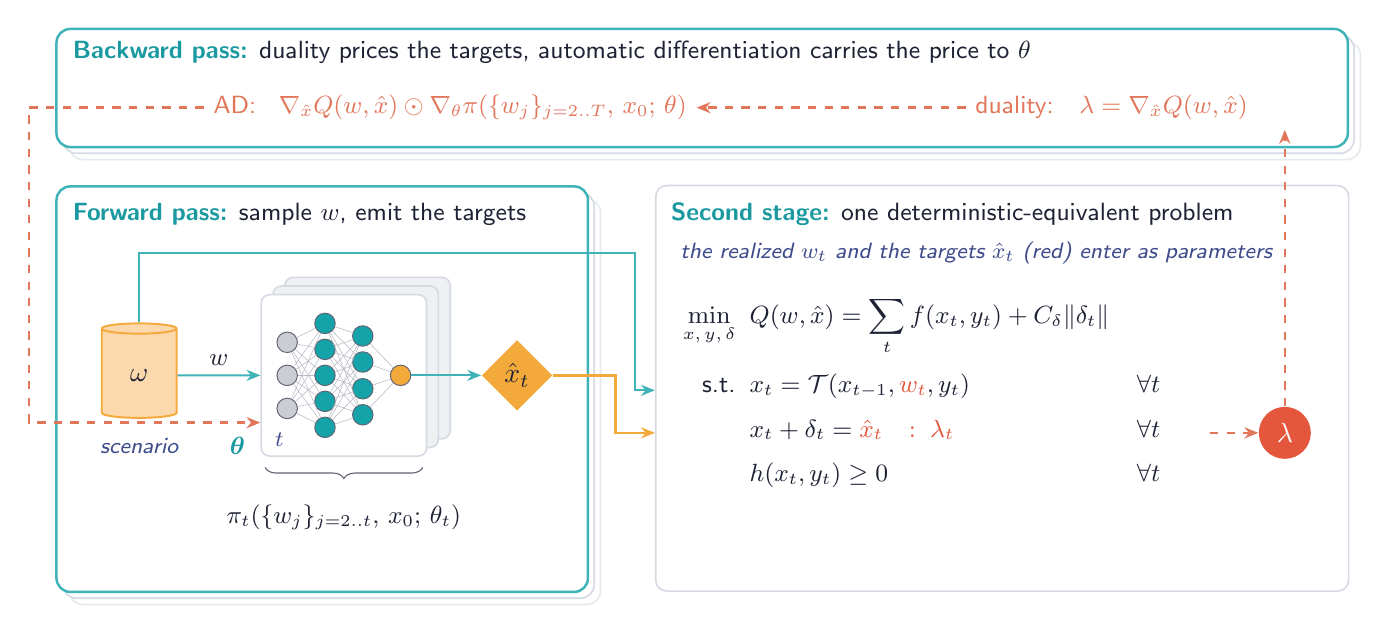
\begin{tikzpicture}
  % ---- backward pass band (top) ----
  \lane{0}{5.65}{16.4}{7.15}
  \node[title] at (0.2,6.85) {\textcolor{dTeal}{\bfseries Backward pass:} \textcolor{dInk}{duality prices the targets, automatic differentiation carries the price to $\theta$}};
  \node[font=\small,text=dCoral] (ad) at (5.0,6.15) {AD:\;\; $\nabla_{\xh}Q(w,\xh)\odot\nabla_\theta\polT$};
  \node[font=\small,text=dCoral] (du) at (13.4,6.15) {duality:\;\; $\lambda=\nabla_{\xh}Q(w,\xh)$};
  \draw[dual] (du.west) -- (ad.east);

  % ---- forward pass (bottom left) ----
  \lane{0}{0}{6.75}{5.15}
  \node[title] at (0.2,4.8) {\textcolor{dTeal}{\bfseries Forward pass:} \textcolor{dInk}{sample $w$, emit the targets}};
  \node[store] (om) at (1.05,2.75) {$\omega$};
  \node[note] at (1.05,1.85) {scenario};
  \policy{3.65,2.75}{p}
  \draw[fwd] (om.east) -- node[above,font=\small] {$w$} (pin2.west -| psheet.west);
  \node[dia] (xh) at (5.85,2.75) {$\xh_t$};
  \draw[fwd] (pout.east) -- (xh.west);
  \draw[decorate,decoration={brace,mirror,amplitude=4pt},dInk!70] (2.65,1.58) -- (4.65,1.58);
  \node[font=\small] at (3.65,0.95) {$\pol$};

  % ---- the deterministic equivalent (bottom right) ----
  \node[card,minimum width=8.8cm,minimum height=5.15cm,anchor=south west] (de) at (7.6,0) {};
  \node[title] at (7.8,4.8) {\textcolor{dTeal}{\bfseries Second stage:} \textcolor{dInk}{one deterministic-equivalent problem}};
  \node[note,anchor=west] at (7.8,4.3) {the realized $w_t$ and the targets $\xh_t$ (red) enter as parameters};
  \node[anchor=north west,font=\small,inner sep=0pt] (pb) at (7.95,3.75) {\problem};
  % targets and scenario into the problem (rows: dynamics y=\rowT, target y=\rowX)
  \def\rowT{2.56}\def\rowX{2.02}
  \draw[tgt] (xh.east) -- (7.1,2.75) -- (7.1,\rowX) -- (7.6,\rowX);
  \draw[fwd] (om.north) |- (7.35,4.3) -- (7.35,\rowT) -- (7.6,\rowT);

  % ---- returns ----
  \node[lnode] (lam) at (15.6,\rowX) {$\lambda$};
  \draw[dual] (14.65,\rowX) -- (lam.west);
  \draw[dual] (lam.north) -- (lam.north |- du.south);
  \draw[dual] (ad.west) -| (-0.35,2.15) -- (psheet.west |- 0,2.15);
  \node[font=\small\bfseries,text=dTeal] at (2.3,1.85) {$\bm\theta$};
\end{tikzpicture}
\fi
\end{document}
